% Options for packages loaded elsewhere
\PassOptionsToPackage{unicode}{hyperref}
\PassOptionsToPackage{hyphens}{url}
\PassOptionsToPackage{dvipsnames,svgnames,x11names}{xcolor}
%
\documentclass[
  10pt,
  dvipsnames,enabledeprecatedfontcommands]{scrartcl}
\title{Weight Chapter Outline}
\author{}
\date{\vspace{-2.5em}9/1/2022}

\usepackage{amsmath,amssymb}
\usepackage{lmodern}
\usepackage{iftex}
\ifPDFTeX
  \usepackage[T1]{fontenc}
  \usepackage[utf8]{inputenc}
  \usepackage{textcomp} % provide euro and other symbols
\else % if luatex or xetex
  \usepackage{unicode-math}
  \defaultfontfeatures{Scale=MatchLowercase}
  \defaultfontfeatures[\rmfamily]{Ligatures=TeX,Scale=1}
\fi
% Use upquote if available, for straight quotes in verbatim environments
\IfFileExists{upquote.sty}{\usepackage{upquote}}{}
\IfFileExists{microtype.sty}{% use microtype if available
  \usepackage[]{microtype}
  \UseMicrotypeSet[protrusion]{basicmath} % disable protrusion for tt fonts
}{}
\usepackage{xcolor}
\IfFileExists{xurl.sty}{\usepackage{xurl}}{} % add URL line breaks if available
\IfFileExists{bookmark.sty}{\usepackage{bookmark}}{\usepackage{hyperref}}
\hypersetup{
  pdftitle={Weight Chapter Outline},
  colorlinks=true,
  linkcolor={Maroon},
  filecolor={Maroon},
  citecolor={Blue},
  urlcolor={blue},
  pdfcreator={LaTeX via pandoc}}
\urlstyle{same} % disable monospaced font for URLs
\usepackage{graphicx}
\makeatletter
\def\maxwidth{\ifdim\Gin@nat@width>\linewidth\linewidth\else\Gin@nat@width\fi}
\def\maxheight{\ifdim\Gin@nat@height>\textheight\textheight\else\Gin@nat@height\fi}
\makeatother
% Scale images if necessary, so that they will not overflow the page
% margins by default, and it is still possible to overwrite the defaults
% using explicit options in \includegraphics[width, height, ...]{}
\setkeys{Gin}{width=\maxwidth,height=\maxheight,keepaspectratio}
% Set default figure placement to htbp
\makeatletter
\def\fps@figure{htbp}
\makeatother
\setlength{\emergencystretch}{3em} % prevent overfull lines
\providecommand{\tightlist}{%
  \setlength{\itemsep}{0pt}\setlength{\parskip}{0pt}}
\setcounter{secnumdepth}{5}
\newlength{\cslhangindent}
\setlength{\cslhangindent}{1.5em}
\newlength{\csllabelwidth}
\setlength{\csllabelwidth}{3em}
\newlength{\cslentryspacingunit} % times entry-spacing
\setlength{\cslentryspacingunit}{\parskip}
\newenvironment{CSLReferences}[2] % #1 hanging-ident, #2 entry spacing
 {% don't indent paragraphs
  \setlength{\parindent}{0pt}
  % turn on hanging indent if param 1 is 1
  \ifodd #1
  \let\oldpar\par
  \def\par{\hangindent=\cslhangindent\oldpar}
  \fi
  % set entry spacing
  \setlength{\parskip}{#2\cslentryspacingunit}
 }%
 {}
\usepackage{calc}
\newcommand{\CSLBlock}[1]{#1\hfill\break}
\newcommand{\CSLLeftMargin}[1]{\parbox[t]{\csllabelwidth}{#1}}
\newcommand{\CSLRightInline}[1]{\parbox[t]{\linewidth - \csllabelwidth}{#1}\break}
\newcommand{\CSLIndent}[1]{\hspace{\cslhangindent}#1}
%\documentclass{article}

% %packages
 \usepackage{booktabs}
\usepackage{subcaption}
\usepackage{multirow}
\usepackage{colortbl}
\usepackage{graphicx}
\usepackage{longtable}
\usepackage{ragged2e}
\usepackage{etex}
%\usepackage{yfonts}
\usepackage{marvosym}
\usepackage[notextcomp]{kpfonts}
\usepackage{nicefrac}
\newcommand*{\QED}{\hfill \footnotesize {\sc Q.e.d.}}
\usepackage{floatrow}
%\usepackage[titletoc]{appendix}
%\renewcommand\thesubsection{\Alph{subsection}}

\usepackage[textsize=footnotesize]{todonotes}
\newcommand{\ali}[1]{\todo[color=gray!40]{#1}}
\newcommand{\mar}[1]{\todo[color=blue!40]{#1}}
\newcommand{\raf}[1]{\todo[color=olive!40]{#1}}
%\linespread{1.5}
\newcommand{\indep}{\!\perp \!\!\! \perp\!}


\setlength{\parindent}{10pt}
\setlength{\parskip}{1pt}


%language
\usepackage{times}
\usepackage{t1enc}
%\usepackage[utf8x]{inputenc}
%\usepackage[polish]{babel}
%\usepackage{polski}




%AMS
\usepackage{amsfonts}
\usepackage{amssymb}
\usepackage{amsthm}
\usepackage{amsmath}
\usepackage{mathtools}

\usepackage{geometry}
 \geometry{a4paper,left=35mm,top=20mm,}


%environments
\newtheorem{fact}{Fact}



%abbreviations
\newcommand{\ra}{\rangle}
\newcommand{\la}{\langle}
\newcommand{\n}{\neg}
\newcommand{\et}{\wedge}
\newcommand{\jt}{\rightarrow}
\newcommand{\ko}[1]{\forall  #1\,}
\newcommand{\ro}{\leftrightarrow}
\newcommand{\exi}[1]{\exists\, {_{#1}}}
\newcommand{\pr}[1]{\mathsf{P}(#1)}
\newcommand{\cost}{\mathsf{cost}}
\newcommand{\benefit}{\mathsf{benefit}}
\newcommand{\ut}{\mathsf{ut}}

\newcommand{\odds}{\mathsf{Odds}}
\newcommand{\ind}{\mathsf{Ind}}
\newcommand{\nf}[2]{\nicefrac{#1\,}{#2}}
\newcommand{\R}[1]{\texttt{#1}}
\newcommand{\prr}[1]{\mbox{$\mathtt{P}_{prior}(#1)$}}
\newcommand{\prp}[1]{\mbox{$\mathtt{P}_{posterior}(#1)$}}

\newcommand{\s}[1]{\mbox{$\mathsf{#1}$}}


\newtheorem{q}{\color{blue}Question}
\newtheorem{lemma}{Lemma}
\newtheorem{theorem}{Theorem}



%technical intermezzo
%---------------------

\newcommand{\intermezzoa}{
	\begin{minipage}[c]{13cm}
	\begin{center}\rule{10cm}{0.4pt}



	\tiny{\sc Optional Content Starts}
	
	\vspace{-1mm}
	
	\rule{10cm}{0.4pt}\end{center}
	\end{minipage}\nopagebreak 
	}


\newcommand{\intermezzob}{\nopagebreak 
	\begin{minipage}[c]{13cm}
	\begin{center}\rule{10cm}{0.4pt}

	\tiny{\sc Optional Content Ends}
	
	\vspace{-1mm}
	
	\rule{10cm}{0.4pt}\end{center}
	\end{minipage}
	}
%--------------------






















\newtheorem*{reply*}{Reply}
\usepackage{enumitem}
\newcommand{\question}[1]{\begin{enumerate}[resume,leftmargin=0cm,labelsep=0cm,align=left]
\item #1
\end{enumerate}}

\usepackage{float}

% \setbeamertemplate{blocks}[rounded][shadow=true]
% \setbeamertemplate{itemize items}[ball]
% \AtBeginPart{}
% \AtBeginSection{}
% \AtBeginSubsection{}
% \AtBeginSubsubsection{}
% \setlength{\emergencystretch}{0em}
% \setlength{\parskip}{0pt}






\usepackage[authoryear]{natbib}

%\bibliographystyle{apalike}



\usepackage{tikz}
\usetikzlibrary{positioning,shapes,arrows}

\ifLuaTeX
  \usepackage{selnolig}  % disable illegal ligatures
\fi

\begin{document}
\maketitle

{
\hypersetup{linkcolor=}
\setcounter{tocdepth}{2}
\tableofcontents
}
\hypertarget{introduction}{%
\section{Introduction}\label{introduction}}

Consider two different items of match evidence:\footnote{These are
  stylized after two items of evidence in the notorious Wayne Williams
  case. Probabilities have been slightly but not unrealistically shifted
  to be closer to each other to make a conceptual point. The original
  probabilities were 1/100 for the dog fur, and 29/1148 for Wayne
  Williams' hair.} The suspects dog's fur matches the dog fur found in a
carpet wrapped around one of the bodies (\textsf{dog}). A hair found on
one of the victims matches that of the suspect (\textsf{hair}). What are
the fact-finders to make of this evidence? To start with, some
probabilistic evaluation thereof should be useful.

Accordingly, an expert testifies that the probability of a random
person's hair matching the reference sample is 0.0252613, and it so
happens that the probability of a random dog's hair matching the
reference sample is very close, 0.025641. You assume that the
probabilities of matches if the suspect (respectively, the suspect's
dog) is the source is one, and that these probabilities of a match are
independent of each other conditional on either truth value of the
source hypothesis (\(\mathsf{source}\) and \(\neg \mathsf{source}\)).
Then, to evaluate the total impact of the evidence on the source
hypothesis you calculate: \begin{align*}
\pr{\s{dog}\wedge \s{hair} \vert \neg \s{source}} & = \pr{\s{dog} \vert \neg \s{source}} \times \pr{\s{hair} \vert \neg \s{source}} \\
& =  0.0252613 \times  0.025641 = \ensuremath{6.4772626\times 10^{-4}}
\end{align*} This seems like a low number. To get a better grip on how
this should be interpreted, the expert shows you how the posterior
depends on the prior, given this evidence (Figure
\ref{fig:impactOfPoint}. The posterior of .99 is reached as soon as your
prior is higher than 0.061.

\begin{figure}[H]


\begin{center}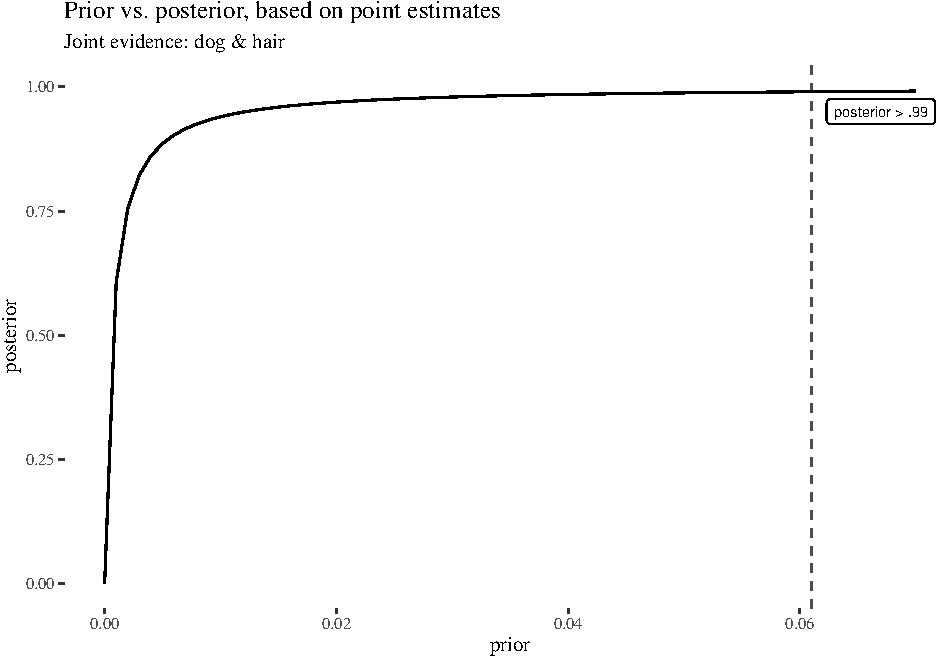
\includegraphics[width=0.8\linewidth]{chapter-outline_files/figure-latex/impactOfPoint4-1} \end{center}

\caption{Impact of dog fur and human hair evidence on the prior, point estimates.}

\label{fig:impactOfPoint}

\end{figure}

While perhaps not sufficient for conviction, the evidence seems pretty
solid: a minor additional piece of evidence could tip the scale. But
then, you reflect on what you have been told and ask the expect:
\emph{wait, but how do you know these exact point probabilities? There must be some aleatory uncertainties around these estimates, and we should pay attention to these!}
The expert agrees, and tells you that in fact the hair evidence estimate
is based on 29 matches found in a database of size 1148, and the dog
evidence estimate was based on finding two matches in a reference class
of size 78.

Well, that means the point estimates did not tell us the whole story,
you think. What to do next? You might try to factor what you have been
just told into your evaluation, but unless you have some training in
probability, you might have hard time doing this correctly. So instead,
you push the expert further:
\emph{well, with a 99\% margin of errors, what are the ranges for these estimates, what are the worst-case and best-case scenarios?}
The expert thinks for a while about giving you confidence intervals, but
abandons this idea, as they are deeply problematic.\footnote{We
  discussed this in a previous chapter XXX.} So instead, he decides to
tell you what the credible intervals are. He says:
\emph{if we start with uniform priors, then the  highest posterior density ranges in which the true frequencies lie with posterior probability of .99 are (.015,.037) for hair and (.002, .103) for fur.}

With good intentions, you calculate the estimate that is the most
charitable to the suspect.
\(\mathsf{P}_{char}(\s{dog}\wedge \s{hair} \vert \neg \s{source}) = .037 * .103 =.003811\).
This number is around 5.88 times greater than the original estimate! You
ask what the impact of evidence on the prior would be given this
scenario, and the answer is that now the prior needs to be higher than
0.274 for the posterior to be above .99 (Figure
\ref{fig:impactOfCharitable}). You are not convinced that the evidence
is fairly strong anymore.

\begin{figure}[H]


\begin{center}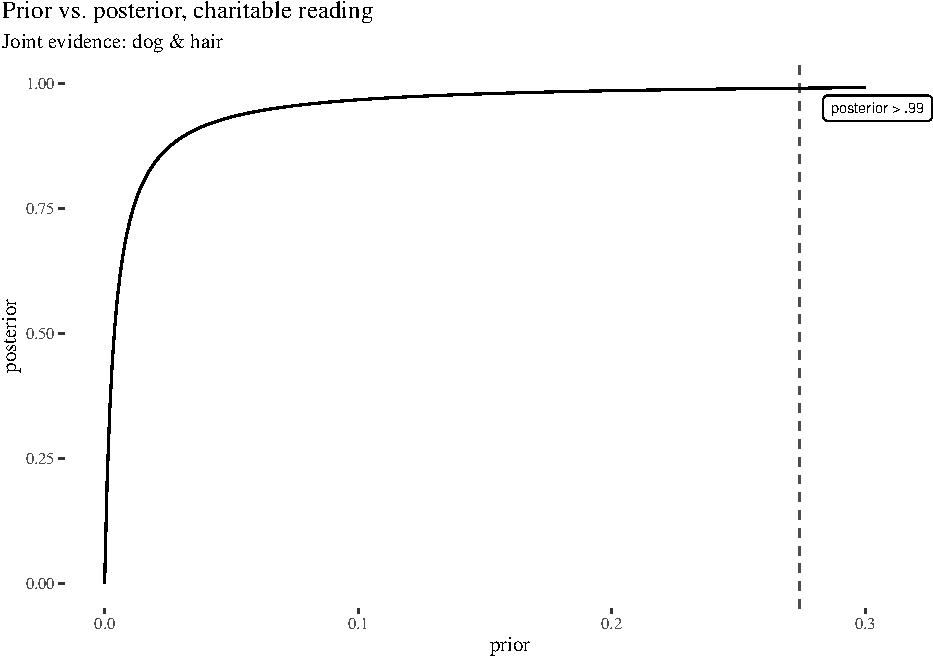
\includegraphics[width=0.8\linewidth]{chapter-outline_files/figure-latex/fig:charitableImpact7-1} \end{center}

\caption{Impact of dog fur and human hair evidence on the prior, charitable reading.}

\label{fig:impactOfCharitable}

\end{figure}

But you made an important blunder. Just because the worst-case
probability estimate for one event is \(x\) and the worst-case
probability estimate for another independent event is \(y\), it does not
follow that the worst-case probability estimate for their conjunction is
\(xy\), if the margin of error is kept fixed. The intuitive reason is
quite simple: just because the probability of an extreme (or larger
absolute) value \(x\) for one variable is .01, and so it is for the
value \(y\) of another independent variable, it does not follow that the
probability that those two independent variables take values \(x\) and
\(y\) simultaneously is the same. This probability is actually much
smaller.

In fact, if you knew what distributions the expert used (it should have
been beta distributions in this context), you could work your way back
and calculate the .99 highest posterior density interval for the
conjunction, which is \((0.000023, 0.002760)\). The proper charitable
reading would then require the prior to be above .215 for the posterior
to be above .99. Still not enough to convict, but at least now we worked
out the consequences of the aleatory uncertainties involved provided the
margin of error is fixed. Is this good enough?

Well, it seems the interval presentation instead of doing us good led us
into error --- the general phenomenon is that intervals do \textbf{not}
contain enough information to reliably reason about such things as
reliability, margins of errors and so on. Even if we are happy with the
interval that we obtained, we won't be able to correctly obtain a new
interval once a new item of evidence is included. That is, unless we
proceed through the densities.

Another problem is that looking at intervals might be useful if the
underlying distributions are fairly symmetrical. But in our case, they
might not be. For instance, Figure \ref{fig:densities} illustrates are
the beta densities for dog fur and human hair, together with
sampling-approximated density for the joint evidence. Crucially, the
distribution is not symmetric, and so switching the margin of error
moves the right edge of the interval much faster towards lower values.
If you were only informed about the edges of the interval, you would be
oblivious to such phenomena and the fact that the most likely value does
\textbf{not} simply lie in the middle between the edges of the interval.

\begin{figure}[H]


\begin{center}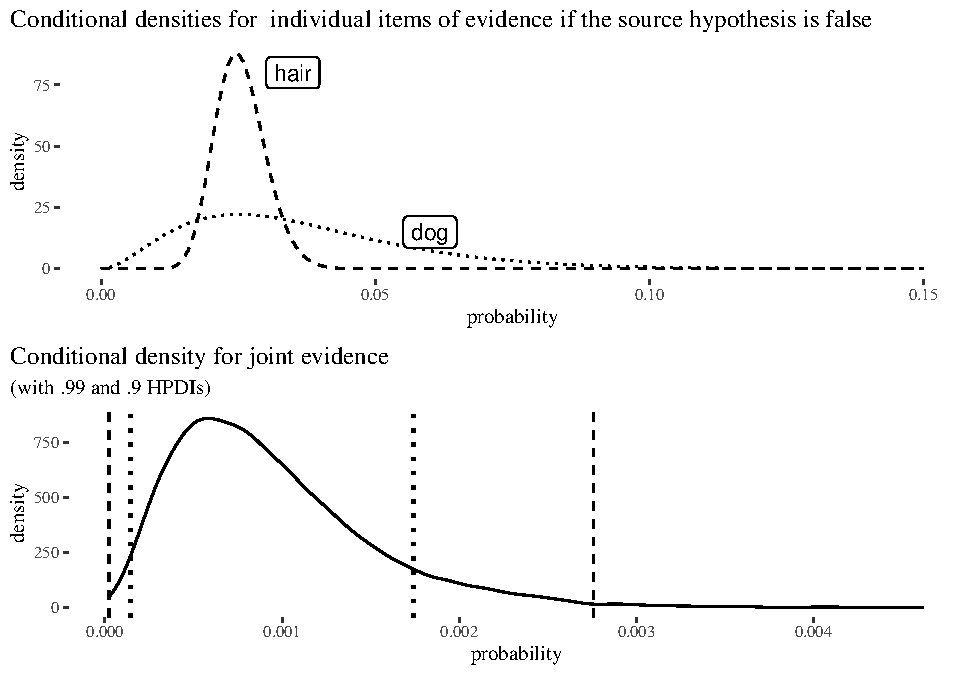
\includegraphics[width=0.8\linewidth]{chapter-outline_files/figure-latex/fig:densities-1} \end{center}

\caption{Beta densities for individual items of evidence and the resulting joint density with .99 and .9 highest posterior density intervals, assuming the sample sizes as discussed and independence, with uniform priors.}

\label{fig:densities}

\end{figure}

This means that a better representation of the uncertainty involving the
dependence of the posterior on the prior involves multiple possible
lines whose density mirrors the density around the probability of the
evidence (Figure \ref{fig:lines}).

\begin{figure}[H]


\begin{center}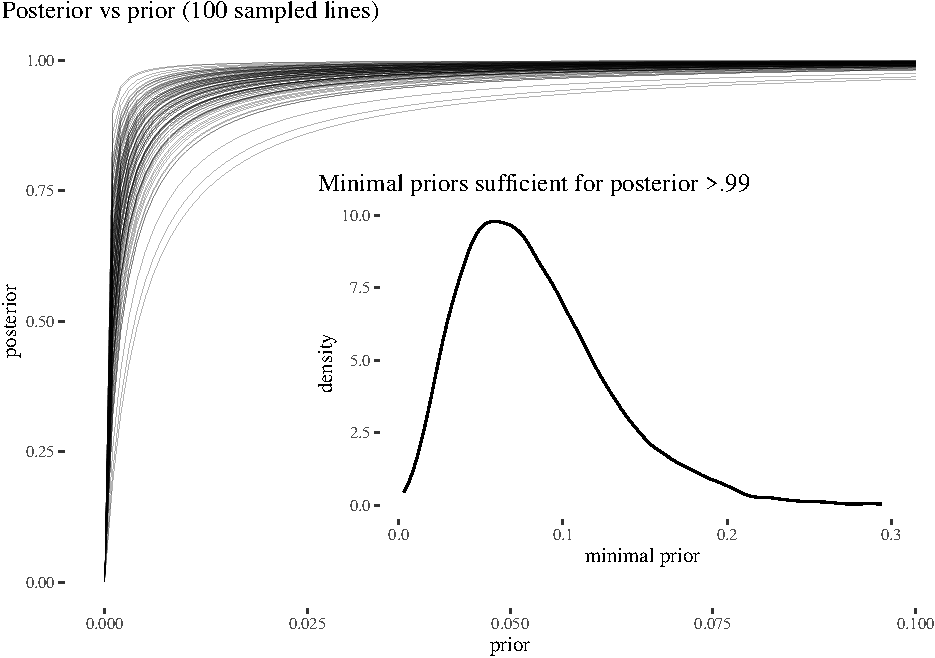
\includegraphics[width=0.8\linewidth]{chapter-outline_files/figure-latex/fig:lines3-1} \end{center}

\caption{100 lines illustrating the uncertainty about the dependence of the posterior on the prior given aleatory uncertainty about the evidence, with the distribution of the minimal priors required for the posterior to be above .99.}

\label{fig:lines}

\end{figure}

This is the gist of our chapter: whenever honest density estimates are
available (and they should be available for match evidence evaluation
methods whose reliability has been properly studies), it is those
densities that should be reported and used in further reasoning. This
avoids hiding actual aleatory uncertainties under the carpet, and allows
for more correct reasoning where interval-based representation might
either lead one astray or leave one oblivious to important probabilistic
considerations.

The rest of this chapter expands on this idea in a few dimensions.
First, it places it in the context of philosophical discussions
surrounding a proper probabilistic representation of uncertainty. The
main alternatives on the market are precise probabilism and imprecise
probabilism. We argue that both options are problematic and should be
superseded by the second-order representation. Second,

\hypertarget{three-probabilisms}{%
\section{Three probabilisms}\label{three-probabilisms}}

This section outlines three version of probabilism: precise, imprecise
and higher-order. Precise probabilism, as the name suggests, posits that
an agent' credal state is modeled by a single, precise probability
measure. Imprecise probabilism replaces precise probabilities by sets of
probability measures, while higher-order probabilism relies on
distributions over probability measures. There are good reasons to
abandon precise probabilism and endorse higher-order probabilism.
Imprecise probabilism is a step in the right direction, but as we will
see, it suffers from too many difficulties of its own.

\hypertarget{precise-probabilism}{%
\subsection{Precise Probabilism}\label{precise-probabilism}}

\textbf{Precise probabilism} (\textsf{PP}) holds that a rational agent's
uncertainty about a hypothesis \(H\) is to be represented as a single,
precise probability measure. This is an elegant and simple theory. But
representing our uncertainty about a proposition in terms of a single,
precise probability runs into a number of difficulties. Precise
probabilism fails to capture an important dimension of how our
uncertainty connects with the evidence we have or have not obtained. For
consider this example:

\begin{quote}
\textbf{No evidence v. fair coin}
You hold a coin in your hands but have no evidence 
whatsoever about its bias. You are completely ignorant. Compare this situation with when 
you start tossing the coin and observe the outcome of ten tosses, 
half of which turn out to be heads and half of which turns out to be tails. 
That half of the outcomes were heads is some evidence that the coin is fair: its 
real bias should be be around .5.
\end{quote}

\noindent How do you represent your stances before and after the
observations? Precise probabilism has difficulties modeling the
difference between the two situations. If you deploy the principle of
insufficient evidence, you would start with \(\mathsf{P}_0(H)=.5\) and
end with \(\mathsf{P}_1(H)=.5\), as if nothing changed. If you do not
deploy the principle of insufficient evidence, what do you do?

Precise probabilism runs into trouble even without complete lack of
evidence. An example from the 1872 manuscript `The Fixation of Belief'
(W3 295) by C. S. Peirce makes this clear:

\begin{quote} \textbf{Peirce's beans:} When we have drawn a thousand times, if about half [of the beans] have been white, we have great confidence in this result  ... a confidence which would be entirely wanting if, instead of sampling the bag by 1000 drawings, we had done so by only two.
\end{quote}

\noindent The difficulty for precise probabilism is this. Your best
estimate of the probability of `the next bean will be white' is .5 if
half of the beans you have drawn randomly so far have been white, no
matter whether you have drawn a thousand or only two of them. There is
an intuitive difference between the two cases, but expressing one's
uncertainty with a precise probability does not capture it.\footnote{Similar
  remarks can be found in Peirce's 1878 \emph{Probability of Induction}.
  There, he also proposes to represent uncertainty by at least two
  numbers, the first depending on the inferred probability, and the
  second measuring the amount of knowledge obtained; as the latter,
  Peirce proposed to use some dispersion-related measure of error (but
  then suggested that an error of that estimate should also be estimated
  and so, so that ideally more numbers representing errors would be
  needed).}

Both examples---Peirce's bean example and the earlier one about lack of
evidence---suggest that precise probabilism is not appropriately
responsive to evidence. It ends up assigning a probability of .5 to
situations in which one's evidence is quite different: when no evidence
is available about the coin's bias; when there is little evidence that
the coin is fair (say, after only 2 draws); when there is strong
evidence that the coin is fair (say, after 1000 draws).\footnote{Precise
  probabilism suffers from other difficulties. For example it has
  problems with formulating a sensible method of probabilistic opinion
  aggregation Stewart \& Quintana (2018). A seemingly intuitive
  constraint is that if every member agrees that \(X\) and \(Y\) are
  probabilistically independent, the aggregated credence should respect
  this. But this is hard to achieve if we stick to PP (Dietrich \& List,
  2016). For instance, a \emph{prima facie} obvious method of linear
  pooling does not respect this. Consider probabilistic measures \(p\)
  and \(q\) such that \(p(X) = p(Y) = p(X\vert Y) = 1/3\) and
  \(q(X) = q(Y) = q(X\vert Y) = 2/3\). On both measures, taken
  separately, \(X\) and \(Y\) are independent. Now take the average,
  \(r=p/2+q/2\). Then \(r(X\cap Y) = 5/18 \neq r(X)r(Y)=1/4\).}

\hypertarget{imprecise-probabilism}{%
\subsection{Imprecise Probabilism}\label{imprecise-probabilism}}

What if we give up the assumption that probability assignments should be
precise? \textbf{Imprecise probabilism} (\textsf{IP}) holds that an
agent's credal stance towards a hypothesis \(H\) is to be represented by
means of a \emph{set of probability measures}, typically called a
representor \(\mathbb{P}\), rather than a single measure \(\mathsf{P}\).
The representor should include all and only those probability measures
which are compatible (in a sense to be specified) with the evidence. For
instance, if an agent knows that the coin is fair, their credal state
would be captured by the singleton set \(\{\mathsf{P}\}\), where
\(\mathsf{P}\) is a probability measure which assigns \(.5\) to \(H\).
If, on the other hand, the agent knows nothing about the coin's bias,
their credal state would rather be represented by means of the set of
all probabilistic measures, as none of them is excluded by the available
evidence. Note that the set of probability measures does not represent
admissible options that the agent could legitimately pick from. Rather,
the agent's credal state is essentially imprecise and should be
represented by means of the entire set of probability
measures.\footnote{For the development of imprecise probabilism, see
  (Fraassen, 2006; Gärdenfors \& Sahlin, 1982; Joyce, 2005; Kaplan,
  1968; Keynes, 1921; Levi, 1974; Sturgeon, 2008; Walley, 1991),
  (Bradley, 2019) is a good source of literature.}

Imprecise probabilism shares some similarities with what we might call
\textbf{interval probabilism} due to {[}KYBURG
1961{]}\todo{REF Kyburg. Probability and the Logic of Rational Belief. Wesleyan University Press, Middletown Connecticut, 1961 and H. E. Kyburg and C. M. Teng. Uncertain Inference. Cambridge University Press, Cambridge, 2001.}.
On interval probabilism, precise probabilities are replaced by intervals
of probabilities. On imprecise probabilism, instead, precise
probabilities are replaced by sets of probabilities. This makes
imprecise probabilism more general since the probabilities of a
proposition in the representor set do not have to form a closed
interval. Both approaches, however, can model situations of complete
lack of evidence by probability measures that assign values in the
interval {[}0, 1{]}.

As more evidence is gathered, the interval might widen or shrink (in
Kyburg's approach) or some probability measures will be added to, and
others removed from, the representor set (in imprecise probabilism).
Learning is modeled in a somewhat idiosyncratic way in Kyburg's interval
probabilism by performing operations on intervals.\footnote{EXPLAIN} The
advantage of imprecise probabilism, instead, is that it provides a
straightforward picture of learning from evidence, that is a natural
extension of the classical Bayesian approach. This makes imprecise
probabilism much preferable to interval probabilism. When faced with new
evidence \(E\) between time \(t_0\) and \(t_1\), the representor set
should be updated point-wise, running the standard Bayesian updating on
each probability measure in the representor:
\begin{align*} \label{eq:updateRepresentor}
\mathbb{P}_{t_1} = \{\mathsf{P}_{t_1}\vert \exists\, {\mathsf{P}_{t_0} \!\in  \mathbb{P}_{t_0}}\,\, \forall\, {H}\,\, \left[\mathsf{P}_{t_1}(H)=\mathsf{P}_{t_0}(H \vert E)\right] \}.
\end{align*}

\textbf{Marcello's comment: can imprecise probabilism model Peirce's bean example?  Not clear to me. Did not find mention of this in the draft. Seems we need to mention this. Here would be a good place to illustrate how the point-wise updating work in the bean's example.}

Unfortunately, because of this point-wise updating, imprecise
probabilism runs into the problem of \textbf{belief inertia}. (Levi,
1980). Consider again Peirce bean's example. Say you start drawing beans
knowing only that the true proportion of red beans is in the interval
\((0,1)\). \todo{M: open or closed interval?} This models a situation of
lack of evidence. As you draw beans from the urn and discover their
color, you should be able to learn something about the proportion of
colors in the urn. This is not so with imprecise probabilism, however.
For suppose you draw two beans both of which are red. On imprecise
probabilism, your initial credal state is to be modeled by the set of
all possible probability measures over your algebra of propositions.
Once you observe the two beans, each particular measure from your
initial representor gets updated to a different one that assigns a
higher probability to ``red,'' but also each measure in your original
representor can be obtained by updating some other measure in your
original representor on the evidence (and the picture does not change if
you continue with the remaining 2998 observations).
\todo{M: Can this be more clear? Not sure I completely follow...} Thus,
if you are to update your representor point-wise, you will end up with
the same representor set. Consequently, the edges of your resulting
interval will remain the same. In the end, it is not clear how you are
supposed to learn that the proportion of beans is such and
such.\footnote{ Here's another example from (Rinard, 2013). Either all
  the marbles in the urn are green (\(H_1\)), or exactly one tenth of
  the marbles are green (\(H_2\)). Your initial credence \([0,1]\) in
  each. Then you learn that a marble drawn at random from the urn is
  green (\(E\)). After conditionalizing each function in your
  representor on this evidence, you end up with the the same spread of
  values for \(H_1\) that you had before learning \(E\), and no matter
  how many marbles are sampled from the urn and found to be green.}

Some downplay the problem of belief inertia. They insist that vacuous
priors should not be used and that imprecise probabilism gives the right
results when the priors are non-vacuous. After all, if you started with
knowing truly nothing, then perhaps it is right to conclude that you
will never learn anything. Another strategy is to say that, in a state
of complete ignorance, a special updating rule should be
deployed.\footnote{(Elkin, 2017) suggests the rule of
  \emph{credal set replacement} that recommends that upon receiving
  evidence the agent should drop measures rendered implausible, and add
  all non-extreme plausible probability measures. This however, is
  tricky: one needs a separate account of what makes a distribution
  plausible or not. Elkin admits that he has no solution to this: ``But
  how do we determine what the set of plausible probability measures is
  relative to \(E\)? There is no precise rule that I am aware of for
  determining such set at this moment, but I might say that the set can
  sometimes be determined fairly easily'' {[}p.~83{]} He goes on to a
  trivial example of learning that the coin is fair and dropping extreme
  probabilities. This is far from a general account. One also needs a
  principled account of why one should use a separate special update
  rule when starting with complete ignorance.} But no matter what we
think about belief inertia, other problems plague imprecise probabilism.
Two problems are particularly pressing.

\textbf{Marcello's comment: I did not add the bit about how we learn about constraints in imprecise probabilism. Might need to go here as a further difficulty about imprecise probabilism. I could not understand the argment. To be discussed.}

One problem is that imprecise probabilism fails to capture intuitions we
have about evidence and uncertainty in a number of scenarios. Consider
this example:

\begin{quote}
\textbf{Even v. uneven bias:}
\todo{M: embellished example a bit. check! } You have two coins and you know, for sure, that the probability of getting heads is .4, if you toss one coin, and .6, if you toss the other coin. But you do not know which is which. You pick one of the two at random and toss it. You do not know the probability of heads on that toss, but you know it must be either .4 or .6. Contrast this with a case of uneven bias. Say the two coins have different weights, and you have information that the lighter coin is three times more likely to have a .4 bias than a .6 bias. Suppose you pick the lighter coin. So, upon tossing this coin, you should be three times more confident that the probability of getting heads is .4. rather than .6.
\end{quote}

\noindent The first situation can be easily represented by imprecise
probabilism. The representor would contain two probability measures, one
that assigns .4. and the other that assigns .6 to the hypothesis `this
coin lands heads.' But imprecise probabilism cannot represent the second
situation, at least not without moving to higher-order probabilities, in
which case it is no longer clear whether the object-level imprecision
performs any valuable task.\footnote{Other scenarios can be constructed
  in which imprecise probabilism fails to capture distinctive intuitions
  about evidence and uncertainty; see, for example, (Rinard, 2013).
  Suppose you know of two urns, \textsf{GREEN} and \textsf{MYSTERY}. You
  are certain \textsf{GREEN} contains only green marbles, but have no
  information about \textsf{MYSTERY}. A marble will be drawn at random
  from each. You should be certain that the marble drawn from
  \textsf{GREEN} will be green (\(G\)), and you should be more confident
  about this than about the proposition that the marble from
  \textsf{MYSTERY} will be green (\(M\)). In line with how lack of
  information is to be represented on \textsf{IP}, for each
  \(r\in [0,1]\) your representor contains a \(\mathsf{P}\) with
  \(\pr{M}=r\). But then, it also contains one with \(\pr{M}=1\). This
  means that it is not the case that for any probability measure
  \(\mathsf{P}\) in your representor, \(\mathsf{P}(G) > \mathsf{P}(M)\),
  that is, it is not the case that RA is more confident of \(G\) than of
  \(M\). This is highly counter-intuitive.}

Besides descriptive inadequacy, an even deeper, foundantional problem
exists for imprecise probabilism. This problem affects imprecise
probabilism, but not precise probabilism. It arises when we reflect on
the notion of the accuracy of imprecise credal states. A variety of
workable \textbf{scoring rules} for measuring the accuracy of a single
credence function, such as the Brier score, are available. One key
feature that some key candidates have is that they are \emph{proper}:
any agent will score her own credence function to be more accurate than
every other credence function. After all, if an agent thought a
different credence is more accurate, they should switch to it. The
availability of such scoring rules underlies an array of
accuracy-oriented arguments for precise probabilism (roughly, if your
precisse credence follows the axioms of probability theory, no other
credence is going to be more accurate than yours whatever the facts
are). When we turn to imprecise probabilism, there are impossibility
results to the effect that no proper scoring rules are available for
representors. So, as many have noted, the prospects for an
accuracy-based argument for imprecise probabilism look dim
(Campbell-Moore, 2020; Mayo-Wilson \& Wheeler, 2016; Schoenfield, 2017;
Seidenfeld, Schervish, \& Kadane, 2012).

\textbf{Marcello's comment: tried to keep the difficulties for imprecise probabilism to a minimum. Some can go in footnotes. We need to discuss which other difficulties you think should be added, if any, and in what order.}

\hypertarget{higher-order-probabilism}{%
\subsection{Higher order probabilism}\label{higher-order-probabilism}}

There is, however, a view in the neighborhood that fares better: a
second-order perspective.
\todo{Maybe add reference to Jouyce here as well?} In fact, some of the
comments by the proponents of imprecise probabilism go in this
direction. Richard Bradley compares the measures in a representor to
committee members, each voting on a particular issue, say the true
chance or bias of a coin. As they acquire more evidence, the committee
members will often converge on a specific chance hypothesis. Bradley
writes:

\begin{quote}
\dots the committee members are "bunching up". Whatever measure you put over the set of probability functions---whatever "second order probability" you use---the "mass" of this measure gets more and more concentrated around the true chance hypothesis' [BRADLEY p. 157] 
\end{quote}

\noindent Note, however, that such bunching up cannot be modeled by
imprecise probabilism.\footnote{Bradley seems to be aware of that, which
  would explain the use of scare quotes: when he talks about the option
  of using second-order probabilities in decision theory, he insists
  that `there is no justification for saying that there is more of your
  representor here or there.' \textasciitilde{[}p.\textasciitilde195{]}}

And the idea that one should use higher-order probabilities has also
been suggested by critics of imprecise probabilism. For example, Carr
(2020) argues imprecise evidence requires uncertainty about what
credences to have. On Carr's approach, one should use vague credences,
assigning various weights to probabilities---agent's credence in
propositions about either what credences the evidence supports, or about
objective chances. Carr, however, does not articulate this suggestion
more fully and does not explain how her approach would fare against the
difficulties pestering precise ad imprecise probabilism.

Our goal now is to develop a higher-order approach that can handle the
problems that imprecise probabilism runs into. The key idea is that
uncertainty is not a single-dimensional thing to be mapped on a single
one-dimensional scale such as a real line. It is the whole shape of the
whole distribution over parameter values that should be taken under
consideration.\todo{REF}\footnote{Bradley admits this much {[}90{]}, and
  so does Konek in his rejection of locality {[}59{]}. For instance,
  Konek disagrees with: (1) \(X\) is more probable than \(Y\) just in
  case \(p(X)>p(Y)\), (2) \(D\) positively supports \(H\) if
  \(p_D(H)> p(H)\), or (3) \(A\) is preferable to \(B\) just in case the
  expected utility of \(A\) w.r.t. \(p\) is larger than that of \(B\).}
From this perspective, sometimes, when an agent is asked about her
credal stance towards \(X\), they can refuse to summarize it in terms of
a point value \(\mathsf{P}(X)\), instead expressing it in terms of a
probability (density) distribution \(f_x\) treating \(\mathsf{P}(X)\) as
a random variable. Coming back to an example we already argued imprecise
probabilism cannot handle, when the agent knows that the real chance is
either .4 or .6 but the former is three times more likely, she might
refuse to summarize her credal state by saying that
\(\mathsf{PR}(H) = .75 \times .4 + .25 \times .6 = .45\).\footnote{More
  generally, on this perspective, the agent might deny that
  \(\int_{0}^{1} x f(x) \, dx\) is their object-level credence in \(X\),
  if \(f\) is the probability density over possible object-level
  probability values and \(f\) is not sufficiently concentrated around a
  single value for such a one-point summary to do the justice to the
  complexity of the agent's credal state. Whether this expectation
  should be used in betting behavior is a separate problem, here we
  focus on epistemic issues.} This approach in fact lines up with common
practice in Bayesian statistics, where the primary role of uncertainty
representation is assigned to the whole distribution, and summaries such
as the mean, mode standard deviation, mean absolute deviation, or
highest posterior density intervals are only summary ways of
representing the uncertainty involved in a given study, to be used
mostly due to practical restrictions.

From this perspective, the scenarios we discussed---some of which
imprecise probabilism has hard time distinguishing---can be easily
represented in the manner illustrated in Figure
\ref{fig:evidenceResponse}.

\begin{figure}


\begin{center}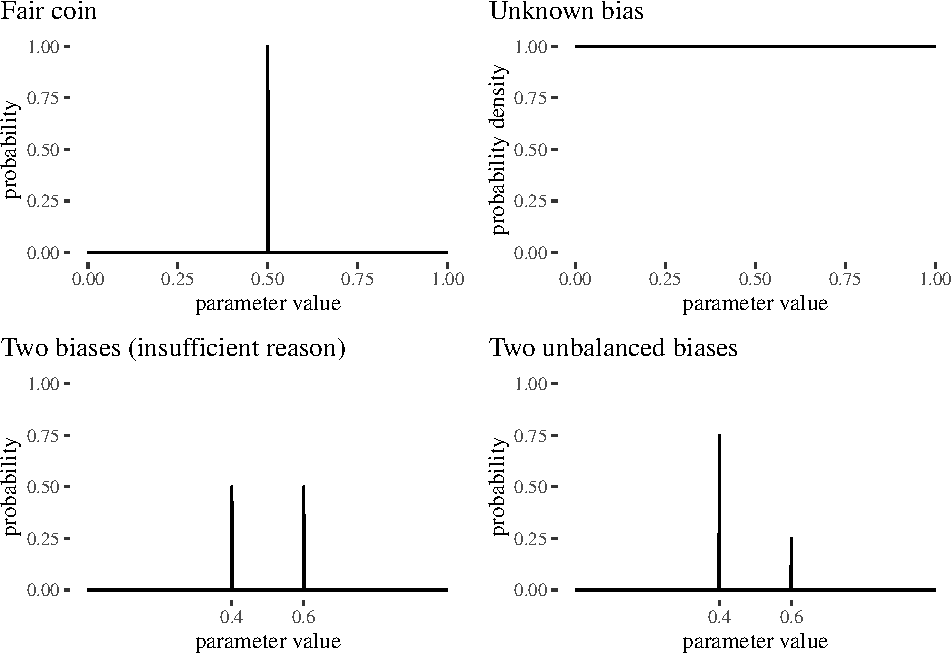
\includegraphics[width=1\linewidth]{chapter-outline_files/figure-latex/fig:evidenceResponse-1} \end{center}
\caption{Examples of RA's distributions responding to various types of evidence for typical cases brought up in the literature.}



\label{fig:evidenceResponse}
\end{figure}

\textbf{Marcello's: Should we say how high order probabilism (1) handles the Peirce's bean example and also (2) how learning is modelled in the higher order approach. I did not see these items (1) clerarly discussed in the draft, there is some discussion of (2), see below, but perhpas it should more upfront? What is the updating rule exactly and how does it differ from the point-wise rule in imprecise probabilism? To be discussed.}

Another difficulty for imprecise probabilism is belief inertia. In the
higher-order probabilism, the problem does not arise, as there is no
problem with modeling learning from observation starting from a uniform
prior. If you just start with a uniform density over \([0,1]\) as your
prior, use binomial probability as likelihood, observing any non-zero
number of heads will exclude 0 and observing any non-zero number of
tails will exclude 1 from the basis of the posterior. Let's see an
example with a grid approximation (\(n=1k\)). For simplicity assume
there are only green and black balls. Our prior is uniform, and then, in
subsequent steps, we observe one green ball, another green ball, and
then a black ball. This is what happens with the posterior as we go
(Figure \ref{fig:intertia2}).

\begin{figure}[H]

\begin{center}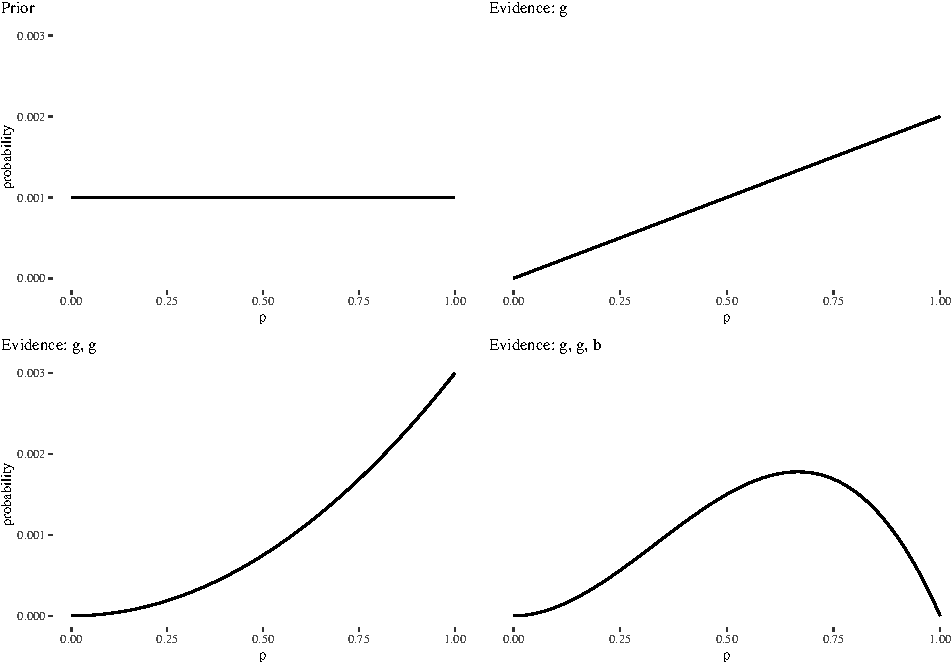
\includegraphics[width=1\linewidth]{chapter-outline_files/figure-latex/fig:inertia2-1} \end{center}
\caption{As observations of green, green and black come in, extreme parameter values drop out of the picture and the posterior is shaped by the evidence.}
\label{fig:intertia2}
\end{figure}

\hypertarget{higher-order-legal-probabilism}{%
\section{Higher-order legal
probabilism}\label{higher-order-legal-probabilism}}

\textbf{Marcello: After coin tossing examples, turn to legal examples that illustrate why high order probabilism outperform precise and impreicse probabilism in legal applications. For simplicity, might be better to separate the more philosohical discussion (previous section) from the legal discussion (this section), or else  things might become too messy too quickly. To be discussed.}

\begin{itemize}



\item[-] Give an example like Peirce's using varying sample sizes to estimate relative proportion of some identifying feature in match evidence, handwriting, genetic profile, fiber, etc. DNA evidence or a simpler form of match evidence (see e.g. the Georgia v. Wayne Williams case) should do here. This can connect back to DNA evidence example in the introduction.\todo{I'm thinking severed fingers, dogs and DNA, will cook up an example preparing for later critical comments about Taroni}



\item[-] The "negation problem" by Cohen (little evidence in favor of H, so Pr(H) is low, cannot mean there is a lot of evidence in favor of not-H, Pr(not-H) is high). 

\end{itemize}

\textbf{Comment:} What is now in \textbf{sections 8}, \textbf{9} and
\textbf{10} should go in these two sections. I would remove all the
stuff about Joyce (since this is about weight), but basically all the
materials we need are in those sections. Also, what is now in
\textbf{section 12} (``Higher order probability and weight in BNs'')
should be part of these two sections.To talk about ``higher ordar
Bayesian networks'' there is not need to introduce all the stuff about
weight. In fact, a reader interested in Bayesian networks might want to
learn about higher order Bayesian networks even though they are not
interested in weight.

\textbf{Possible addition:} To give the reader an intuitive picture, we
could provide three Bayesian networks for the diagnostic example from
the introduction section. The first network has the shape with
\(D \rightarrow T\), and is just how one would do things in the standard
way with sharp probabilities. The second network contains multiple
probability measures about (a) the prior probability of \(D\) and
second-order uncertainty about the error rates that go into the
conditional table for \(P(T | D)\). This is the network using imprecise
probabilism. This is also something like ``sensitivity analysis.''
\todo{Right, but not with the diagnosis; let's use the legal examples to start with}
Finally, the third network contains distributions over multiple
probability distributions---the higher order approach. The same could be
done for the DNA match example. This comparison would convey succinctly
the first major contribution of the chapter. The three Bayesian networks
will also nicely connect with the two motivating examples right at the
start of the chapter. You use the Sally Clark case as an illustration.
This goes even one step further, but it might be good to have a simple
illustration even with a simple match-source Bayesian network.

\hypertarget{weight-of-evidence}{%
\section{Weight of evidence}\label{weight-of-evidence}}

\todo{Yeh, I think in the end this will be another chapter}

The chapter now turns to the weight of evidence and its formalization.

\textbf{Comment:} It is conceptually important to separate the
discussion about precise, imprecise, and higher order probabilism
(previous sections) from weight (this section). Weight of evidence is
one way in which higher order probabilism can be put to use. It can be
confusing to run the discussion of higher order probabilism together
with weight of evidence. Higher order probabilism can still make perfect
sense even if no theory of weight cen be worked out.

\hypertarget{motivating-examples}{%
\subsection{Motivating examples}\label{motivating-examples}}

This section should start with illustrative examples of the
weight/balance distinction and why ``balance alone'' isn't enough to
model the evidential uncertainty relative to a hypothesis of interest.
These examples should be chosen carefully. We can use legal and
non-legal examples. The driving intuition is given by Keynes with the
weight/balance distinction. Some of the examples we saw earlier in
talking about imprecise probabilism can be mentioned here again, such as
(a1) and (a2), and perhaps also (b) and (c).

Upshot is that uncertainty cannot be captured by balance of evidence
alone. There is a further dimension to uncertainty. So we need a theory
that can accommodate this further level of uncertainty. This theory is
essentially the higher order probabilism introduced before.

\hypertarget{desiderata}{%
\subsection{Desiderata}\label{desiderata}}

Here we can discuss monotonicity, completeness, strong increase, etc
(see current \textbf{section 1}). We can list the intuitive properties
(based on the example we presented in both philosophy and law) that any
theory of weight (and perhaps also of completeness/resilience, but on
these notions, see later) should be able to capture. We should try to
keep these requirements as simple as possible and leave complications to
footnotes.

\hypertarget{formal-characterization-of-weight}{%
\subsection{Formal characterization of
weight}\label{formal-characterization-of-weight}}

Higher order probabilism is then put to use to deliver a theory of
weight. What is now in \textbf{section 11} (``Weight of a
distribution'') and \textbf{sections 13} and \textbf{14} ('' Weight of
evidence'' and ``Weights in Bayesian Networks'') forms the bulk of the
theory.

We should also demonstrate that the proposed theory of weight does meet
the intuitive desiderata and can handle the motivating examples. To
better appreciset the novelty of the proposal, It might be interesting
to raise the following questions:

\begin{itemize}

\item[q1] what does a theory of weight based on precise probabilism look like? (maybe it consists of something like Skyrms' resilience or Kaye's completeness, the problem being that these are not measures of weight, but of something else, more on these later)

\item[q2] what does a theory of weight based on imprecise probabilism look like? (is Joyce's theory essentially an attempt to use imprecise probabilism to construct a theory of weight? )\todo{Well, it's a bit funny as Joyce's weight uses precise chance hypotheses instead of IP, so hard to say}

\item[q3] what does a theory of weight based on higher order probabilism look like?

\end{itemize}

Here we are defending a theory fo weight based on higher order
probabilism, but it is interesting to contrast it with a theory of
weight based on the other version of legal probabilism. Here we can also
show why Joyce's theory of weight does not work (either in the main text
or a footnote).

\textbf{Comment:} The current exposition in chapter 11, 13 and 14,
however, is complicated---perhaps overly so. The move from ``weight of a
distribution'' to ``weight of evidence'' is not intuitive and can
confuse the reader. Is there a simpler story to be told here? I think
so. See below.
\todo{Brilliant, I think I can start talking about conditional probabilities to begin with}

\textbf{Suggestion:} There seems to be a nice symmetry. Start with
precise probabilism. We can use sharp probability theory to offer a
theory of the value of the evidence (i.e.~likelihood ratio). Actually, I
think that the likelihood ratio model the idea of balance of the
evidence. What Keynes distinction weight/balance shows is that
likelihood ratio are not, by themselves, enough to model the value of
the evidence. The straightforward move here seems to just have
\textbf{higher order likelihood ratios}. Wouldn't higher order
likelihood ratio be essentially your formal model of the weight of the
evidence? Your measure of weight tracks the difference between (the
weight of the) prior distribution (and the weight of the) posterior
distribution. But higher order likelihood ratios essentially do the same
thing, just like precise likelihood ratios track the difference between
prior and posterior. Is this right? \todo{Yup, more or less}

\textbf{Comment:} If weight if measured by higher order likelihood
ratios, then this can be seen as a generalization of thoughts that many
other had -- say that the absolute value of the likelihood ratio is a
measure of weight (Nance, Glenn Shafer) or that likelihood ratio must be
a measure of weight (Good; see current \textbf{section 4}). So I think
using ````higher order likelihood ratio'' could be a more appealing way
to sell the idea of weight of evidence since most people are already
familiar with likelihood ratios.

\hypertarget{limits-of-our-contribution}{%
\subsection{Limits of our
contribution}\label{limits-of-our-contribution}}

Work by Nance of Dahlman suggests that ``weight'' should play a role in
the standard of proof. We do not take a position on that. Weight could
be regulated by legal rules at the level of rules of decision, rule of
evidence, admissibility, sanctions at the appellate level. All that
matters to us is that, in general, legal decision-making is sensitive to
these further levels of uncertainty (quantity, completeness,
resilience), but whether this should be codified at the level of the
standard of proof or somewhere else, we are not going to take a stance
on that.

\hypertarget{objection}{%
\subsection{Objection}\label{objection}}

Ronald Allen or Bart Verheij might object as follows. Precise
probabilism is bad because we do not always have the numbers we need to
plug into the Bayesian network. Imprecise probabilism partly addresses
this problem by allowing for a range instead of precise numbers. How
does higher order probabilism help address the practical objection that
we often we do not have the numbers we need to plug into the Bayesian
network?

\hypertarget{completeness-and-resilience}{%
\section{Completeness (and
resilience?)}\label{completeness-and-resilience}}

Next the chapter turns to notions related to the weight of evidence,
such as completeness (and perhaps resilience as well). See current
\textbf{sections 5} and \textbf{6}.

\hypertarget{motivating-example}{%
\subsection{Motivating example}\label{motivating-example}}

Give an example using completeness of evidence (pick one or more court
cases). The court case we can use is Porter v. City of San Francisco
(see file with Marcello's
notes).\footnote{This is a wrongful death case in which victim was committed to a hospital facility, but escaped and then died under unclear circumstances. So the nurses and other hospital workers---actually, the city of San Francisco---are accused of contributing to this person's death. Need to check exact accusation---this is not a criminal case. A phone call was made to social services shortly after the person disappeared, but its content was erased from hospital records. Court agrees that content of phone call would be helpful to understand what happened and to assess the credibility of hospital's workers ("The Okupnik call is the only contemporaneous record of what information was reported to the SFSD about Nuriddin’s disappearance, and could contain facts not otherwise known about her disappearance and CCSF’s response. Additionally, the call is relevant to a jury’s assessment of Okupnik’s credibility"). The court thought that the hospital should have kept records of that call. But court did not think the hospital acted in bad faith or intentionally, so it did NOT issue an "adverse inference instruction" (=the missing evidence was favorable to the party that should have preserved it, but failed to do it).}
The jury is given an instruction that a call recording is missing, but
no instruction whether the call should be assumed to be favorable or
not.

What is the jury supposed to do with this information? If the call could
contain information that is favorable or not, shouldn't the jury simply
ignore the fact that the call recording is missing (Hamer's claim)?
Modelling with Bayesian network might turn out useful. Cite also David
Kaye on the issue of completeness. His claim is that when evidence is
known to be missing, then this information should simply be added as
part of the evidence, which is precisely what the court in Porter does.
But again, once we add the fact that the evidence is missing what is the
evidentiary significance of that? What is te jury supposed to do with
that? Does Pr(H) go up, down or stays the same? Kaye does not
say\ldots{}

\hypertarget{bayesian-network-model}{%
\subsection{Bayesian network model}\label{bayesian-network-model}}

\textbf{Comment} I am thinking that incompleteness is modeled by adding
an evidence node to a Bayesian network but without setting a precise
value for that node, and then see if the updated network yields a
different probability than the previous network without the missing
evidence node. The missing evidence node could be added in different
places and this might changes things. In the Porter case the missing
evidence seems to affect the credibility of the other evidence in the
case, we would have a network like this:
\(H\rightarrow E \leftarrow C\), where \(C\) is the missing evidence
node and \(E\) is the available evidence nose. My hunch is that (see
also our paper on reverse Bayesianiam and unanticipated possibilities)
the addition of this credibility node will affect the probability of the
hypothesis (thus proving Hamer wrong).
\todo{I think this will depend on how the probability of obtaining new evidence given guilt and given innocence are, I will keep thinking about this, we'll move to this once the earlier bits are done}

\hypertarget{expected-weight-model}{%
\subsection{Expected weight model}\label{expected-weight-model}}

\textbf{Question:} If what I say above in the comment is correct, then a
question arises, do we need higher order probabilism to model
completeness?

\textbf{Possible answer:} We can use expected weight (see current
\textbf{section 14}). If the expected weight of an additional item of
evidence is null, that would mean that its addition (not matter the
value the added evidence would take) cannot change the probability of
the hypothesis. If the expected weight is different from zero (pace
Hamer who thinks the expected weight is always null), then the evidence
can change the probability of the hypothesis.

\todo{LR ratio and weight}

\hypertarget{weight-and-accuracy}{%
\section{Weight and accuracy}\label{weight-and-accuracy}}

This section addresses the question, why care about weight?

\hypertarget{conclusion}{%
\section*{Conclusion}\label{conclusion}}
\addcontentsline{toc}{section}{Conclusion}

\hypertarget{refs}{}
\begin{CSLReferences}{1}{0}
\leavevmode\vadjust pre{\hypertarget{ref-bradley2019imprecise}{}}%
Bradley, S. (2019). {Imprecise Probabilities}. In E. N. Zalta (Ed.),
\emph{The {Stanford} encyclopedia of philosophy} ({S}pring 2019).
\url{https://plato.stanford.edu/archives/spr2019/entries/imprecise-probabilities/};
Metaphysics Research Lab, Stanford University.

\leavevmode\vadjust pre{\hypertarget{ref-CampbellMoore2020accuracy}{}}%
Campbell-Moore, C. (2020). \emph{Accuracy and imprecise probabilities}.

\leavevmode\vadjust pre{\hypertarget{ref-Carr2020impreciseEvidence}{}}%
Carr, J. R. (2020). Imprecise evidence without imprecise credences.
\emph{Philosophical Studies}, \emph{177}(9), 2735--2758.
\url{https://doi.org/10.1007/s11098-019-01336-7}

\leavevmode\vadjust pre{\hypertarget{ref-Dietrich2016pooling}{}}%
Dietrich, F., \& List, C. (2016). Probabilistic opinion pooling. In A.
Hajek \& C. Hitchcock (Eds.), \emph{Oxford handbook of philosophy and
probability}. Oxford: Oxford University Press.

\leavevmode\vadjust pre{\hypertarget{ref-Lee2017impreciseEpistemology}{}}%
Elkin, L. (2017). \emph{Imprecise probability in epistemology} (PhD
thesis). Ludwig-Maximilians-Universit{ä}t;
Ludwig-Maximilians-Universität München.

\leavevmode\vadjust pre{\hypertarget{ref-Elkin2018resolving}{}}%
Elkin, L., \& Wheeler, G. (2018). Resolving peer disagreements through
imprecise probabilities. \emph{Noûs}, \emph{52}(2), 260--278.
\url{https://doi.org/10.1111/nous.12143}

\leavevmode\vadjust pre{\hypertarget{ref-VanFraassen2006vague}{}}%
Fraassen, B. C. V. (2006). Vague expectation value loss.
\emph{Philosophical Studies}, \emph{127}(3), 483--491.
\url{https://doi.org/10.1007/s11098-004-7821-2}

\leavevmode\vadjust pre{\hypertarget{ref-Gardenfors1982unreliable}{}}%
Gärdenfors, P., \& Sahlin, N.-E. (1982). Unreliable probabilities, risk
taking, and decision making. \emph{Synthese}, \emph{53}(3), 361--386.
\url{https://doi.org/10.1007/bf00486156}

\leavevmode\vadjust pre{\hypertarget{ref-joyce2005probabilities}{}}%
Joyce, J. M. (2005). How probabilities reflect evidence.
\emph{Philosophical Perspectives}, \emph{19}(1), 153--178.

\leavevmode\vadjust pre{\hypertarget{ref-Kaplan1968decision}{}}%
Kaplan, J. (1968). Decision theory and the fact-finding process.
\emph{Stanford Law Review}, \emph{20}(6), 1065--1092.

\leavevmode\vadjust pre{\hypertarget{ref-keynes1921treatise}{}}%
Keynes, J. M. (1921). \emph{A treatise on probability, 1921}. London:
Macmillan.

\leavevmode\vadjust pre{\hypertarget{ref-Levi1974ideterminate}{}}%
Levi, I. (1974). On indeterminate probabilities. \emph{The Journal of
Philosophy}, \emph{71}(13), 391. \url{https://doi.org/10.2307/2025161}

\leavevmode\vadjust pre{\hypertarget{ref-Levi1980enterprise}{}}%
Levi, I. (1980). \emph{The enterprise of knowledge: An essay on
knowledge, credal probability, and chance}. MIT Press.

\leavevmode\vadjust pre{\hypertarget{ref-Mayo-Wilson2016scoring}{}}%
Mayo-Wilson, C., \& Wheeler, G. (2016). Scoring imprecise credences: A
mildly immodest proposal. \emph{Philosophy and Phenomenological
Research}, \emph{92}(1), 55--78.
\url{https://doi.org/10.1111/phpr.12256}

\leavevmode\vadjust pre{\hypertarget{ref-Rinard2013against}{}}%
Rinard, S. (2013). Against radical credal imprecision. \emph{Thought: A
Journal of Philosophy}, \emph{2}(1), 157--165.
\url{https://doi.org/10.1002/tht3.84}

\leavevmode\vadjust pre{\hypertarget{ref-Schoenfield2017accuracy}{}}%
Schoenfield, M. (2017). The accuracy and rationality of imprecise
credences. \emph{Noûs}, \emph{51}(4), 667--685.
\url{https://doi.org/10.1111/nous.12105}

\leavevmode\vadjust pre{\hypertarget{ref-seidenfeld2012forecasting}{}}%
Seidenfeld, T., Schervish, M., \& Kadane, J. (2012). Forecasting with
imprecise probabilities. \emph{International Journal of Approximate
Reasoning}, \emph{53}, 1248--1261.
\url{https://doi.org/10.1016/j.ijar.2012.06.018}

\leavevmode\vadjust pre{\hypertarget{ref-Stewart2018pooling}{}}%
Stewart, R. T., \& Quintana, I. O. (2018). Learning and pooling, pooling
and learning. \emph{Erkenntnis}, \emph{83}(3), 1--21.
\url{https://doi.org/10.1007/s10670-017-9894-2}

\leavevmode\vadjust pre{\hypertarget{ref-Sturgeon2008grain}{}}%
Sturgeon, S. (2008). Reason and the grain of belief. \emph{No{û}s},
\emph{42}(1), 139--165. Retrieved from
\url{http://www.jstor.org/stable/25177157}

\leavevmode\vadjust pre{\hypertarget{ref-walley1991statistical}{}}%
Walley, P. (1991). \emph{Statistical reasoning with imprecise
probabilities}. Chapman; Hall London.

\end{CSLReferences}

\end{document}
